In fully actuated systems, it is possible to produce a control scheme which asymptotically drives the deviations from some specified time-dependent trajectory to zero. The application of control may be viewed as defining an \textit{output function}, $h(q,t)$, with rank($h$) $= m$, which is identically zero when the trajectory is perfectly regulated, and attempting to maintain $h(q,t) = 0$. In underactuated systems, an analogous output function may be defined, however since rank($h$) $<$ rank($q$), $h = 0$ defines a set of admissible values, rather than a unique value, of $q$. In systems modelled by ordinary differential equations, the maximal internal dynamics of the system under the constraint $h=0$ is called the \textit{zero dynamics} \cite{isidori1995nonlinear}. It is possible to explicitly define the zero dynamics by synchronising all of the generalised coordinates of the underactuated system to a single variable, known as the \textit{phase variable}. The remaining variables are said to be under \textit{virtual constraints}.\\

Walking robots are able to be modelled using ordinary differential equations for the majority of their motion, with the exception of their impact dynamics. We therefore apply virtual constraints over what is labelled the \textit{swing phase}, interspersed with impacts. Thus we produce \textit{hybrid zero dynamics} based upon the swing phase dynamics of the robot coupled with the applied virtual constraints, along with the impact dynamics. In this section, the derivation of hybrid zero dynamics for general underactuation degree one robots is presented along with some useful results for the motion planner.

\subsection{Dynamics of a general underactuated walker}
The general equation of motion of a nonlinear time-invariant physical system may be written as:
\begin{equation}\label{eqn:dynamics}
	M\left(q(t)\right)\ddot{q}(t) + C\left(q(t),\dot{q}(t)\right)\dot{q}(t)
	 + G\left(q(t)\right) = B\left(q(t)\right)u(t)
\end{equation}
where $M\left(q(t)\right)$ is the matrix of inertial terms, $C\left(q(t),\dot{q}(t)\right)$ is the matrix of Coriolis and centrifugal terms, $G\left(q(t)\right)$ is the gradient of the potential field and $B\left(q(t)\right)$ is some matrix which specifies the effect of control inputs $u(t)$. \\

As in \cite{hurmuzlu1994rigid}, we assume that the collisions at each footstep are purely inelastic and the impact map has the following form:
\begin{eqnarray}
	q\left(t^+\right) &=& Rq\left(t^-\right) \label{eqn:impactconfig}\\
	\dot{q}\left(t^+\right) &=& R\Delta\left(q\left(t^-\right)\right)\dot{q}\left(t^-\right) \label{eqn:impactvel}
\end{eqnarray} ~\\

For the underactuated walkers considered in this thesis, $R$ represents a relabelling of coordinates. An example is shown of such relabelling for the simple compass gait walker in Figure~\ref{fig:relabelimpact}.

\begin{figure}[htp]
	\centering
	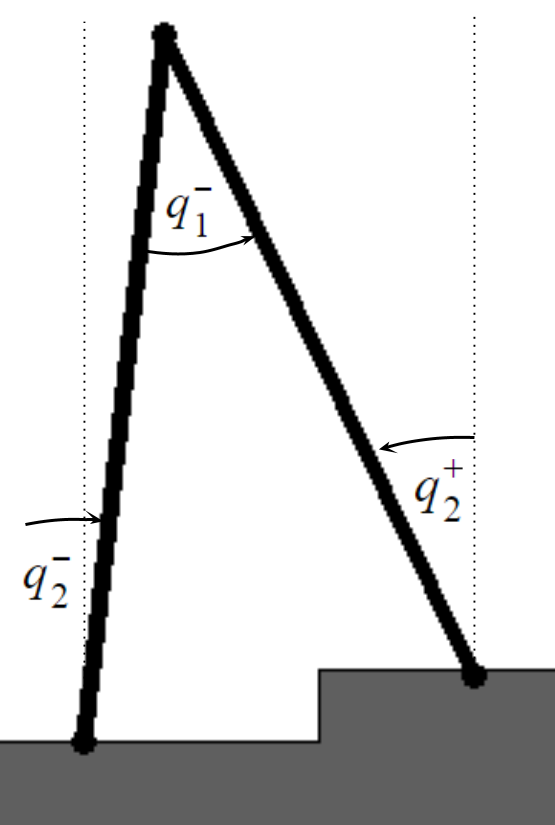
\includegraphics[scale=1]{3TechBackground/impact.png}
	\caption{Change of coordinates at impact}
	\label{fig:relabelimpact}
\end{figure}

\subsection{Application of virtual constraints and zero dynamics}
The application of virtual holonomic constraints is a method by which a system's generalised coordinates may be synchronised to a single coordinate, called the \textit{phase variable}, $\theta$. In order for this to be sensible, we assume that $\theta$ is increasing over some interval $[\theta_0, \theta_n]$. Under that assumption, we may construct functions for all of the generalised coordinates of the form:
\begin{equation}
	q_i(t) = \phi_i\left(\theta(t)\right), ~~ i = 1,2,\ldots,n
\end{equation}
Using trivial differentiation rules, we obtain
\begin{eqnarray}
	\dot{q}_i(t) &=& \frac{\partial\phi_i\left(\theta(t)\right)}{\partial\theta}\dot{\theta},
						~~i = 1,2,\ldots,n \\
	\ddot{q}_i(t) &=& \frac{\partial^2\phi_i\left(\theta(t)\right)}{\partial\theta^2}\dot{\theta}^2 +
						\frac{\partial\phi_i\left(\theta(t)\right)}{\partial\theta}\ddot{\theta},
						~~i = 1,2,\ldots,n
\end{eqnarray}
We define the following vector functions:
\begin{eqnarray}
	\Phi\left(\theta\right) &=& \left[ \phi_1\left(\theta\right), \phi_2\left(\theta\right), \ldots,
	\phi_n\left(\theta\right)\right]^T \\
	\Phi'\left(\theta\right) &=& \left[ \frac{\partial\phi_1\left(\theta\right)}{\partial\theta},
	\frac{\partial\phi_2\left(\theta\right)}{\partial\theta}, \ldots ,
	\frac{\partial\phi_n\left(\theta\right)}{\partial\theta} \right]^T \\
	\Phi''\left(\theta\right) &=& \left[ \frac{\partial^2\phi_1\left(\theta\right)}{\partial\theta^2},
	\frac{\partial^2\phi_2\left(\theta\right)}{\partial\theta^2}, \ldots ,
	\frac{\partial^2\phi_n\left(\theta\right)}{\partial\theta^2} \right]^T
\end{eqnarray} ~\\

Under the assumption perfect regulation of the virtual constraints, thus the above relations holding, we can evaluate the zero dynamics by simple substitution into Equation~\ref{eqn:dynamics}:
\begin{equation}
	M\left(\Phi(\theta)\right)\left[\Phi'(\theta)\ddot{\theta} + \Phi''\dot{\theta}^2\right] + 
	C\left(\Phi(\theta),\Phi'(\theta)\dot{\theta}\right)\Phi'(\theta)\dot{\theta} +
	G\left(\Phi(\theta)\right) = B\left(\Phi(\theta)\right)u_c
\end{equation}
where $u_c$ is the control which achieves perfect regulation of the constraints. This may be rearranged into a more convenient form:
\begin{equation} \label{eqn:zerodyn}
	\alpha(\theta)\ddot{\theta} + \beta(\theta)\dot{\theta}^2 + \gamma(\theta) = 0
\end{equation}
where, if we denote $B^{\perp}(q)$ as a row vector which satisfies $B^{\perp}(q)B(q)u_c = 0$,
\begin{eqnarray}
	\alpha(\theta) &=& B^{\bot}\left(\Phi(\theta)\right)M\left(\Phi(\theta)\right)\Phi'(\theta)\nonumber \\
	\beta(\theta) &=& B^{\bot}\left(\Phi(\theta)\right)\left(M\left(\Phi(\theta)\right)\Phi''(\theta)
		+C\left(\Phi(\theta),\Phi'(\theta)\right)\Phi'(\theta) \right) \nonumber \\
	\gamma(\theta) &=& B^{\bot}\left(\Phi(\theta)\right)G\left(\Phi(\theta)\right)
\end{eqnarray}

\subsection{Partial closed-form solutions for velocity and energy}
One of the useful properties of virtual constraints is the ability that they lend the designer of a motion planner the ability to precompute a partial closed-form solution for velocity and energy. The solution is partial in that we obtain an expression for $\dot{\theta}^2$ in terms of $\theta$ rather than time. Under the assumption that $\theta$ is monotonic, it can be used as a new dependent variable:
\begin{eqnarray}
	\frac{d}{d\theta}\left[\dot{\theta}\left(t(\theta)\right)^2\right] &=& 
	\frac{d}{dt}\frac{dt}{d\theta}\left[\frac{d\theta}{dt}\left(t(\theta)\right)^2\right] \nonumber \\ 
	&=& 2\ddot{\theta}\left(t(\theta)\right)
\end{eqnarray}
Substituting Equation~\ref{eqn:zerodyn} into this expression, we arrive at a first-order ODE in $\dot{\theta}(\theta)^2$:
\begin{equation}\label{eqn:zerodynDE}
	\frac{d}{d\theta}\dot{\theta}(\theta)^2 = -2\frac{\beta(\theta)}{\alpha(\theta)}
		\dot{\theta}(\theta)^2 - 2\frac{\gamma(\theta)}{\alpha(\theta)}
\end{equation}
If we assume, as in \cite{manchester13planning}, that for all $\theta \in [\theta_0, \theta_n]$, we have local instantaneous controllability, i.e. $\alpha(\theta) \neq 0$, then we may solve Equation~\ref{eqn:zerodynDE} numerically over $[\theta_0, \theta_n]$, which yields an affine solution, i.e.
\begin{equation} \label{eqn:affinesoln}
	\dot{\theta}(\theta)^2 = \Gamma(\theta, \theta_0)\dot{\theta}_0^2 + \Psi(\theta, \theta_0)
\end{equation}

For typical walking motions, there exits a single point of maximum potential energy within each footstep. This corresponds to a zero crossing of $\gamma(\theta)$. If we denote this point the \textit{critical velocity}, $\theta_c$, the affine form of Equation \ref{eqn:affinesoln} allows us to trivially determine the feasibility of a particular constraint given the initial velocity; for any given constraint there exists an initial velocity which satisfies
\begin{equation} \label{eqn:critvel}
	\Gamma(\theta_c)\dot{\theta}_{0,c}^2 + \Psi(\theta_c) = 0
\end{equation}
For any initial velocity less than $\dot{\theta}_{0,c}$, there is no real solution for Equation \ref{eqn:affinesoln} at $\theta_c$; the robot will fall back rather than complete the footstep.

Following from Equation \ref{eqn:affinesoln}, we may also derive the total mechanical energy of the system. For general systems with dynamics as expressed in Equation~\ref{eqn:dynamics}, the mechanical energy has the form:
\begin{equation}
	H\left(q,\dot{q}\right) = \dot{q}^TM(q)\dot{q} + V(q)
\end{equation}
Under perfectly regulated virtual constraints, this reduces to:
\begin{equation}
	\bar{H}\left(\theta,\dot{\theta}\right) := \Upsilon(\theta)\dot{\theta}^2 + \Xi(\theta)
\end{equation}
where
\begin{eqnarray*}
	\Upsilon(\theta) &=& \Phi'(\theta)^TM\left(\Phi(\theta)\right)\Phi'(\theta) \\
	\Xi(\theta) &=& V\left(\Phi(\theta)\right)
\end{eqnarray*}
Since this is affine in $\dot{\theta}^2$ for a given $\theta$, we may trivially calculate the closed form:
\begin{equation}
	H\left(\theta, \dot{\theta}\right) =
	\Upsilon(\theta)\Gamma\left(\theta,\theta_0\right)\dot{\theta}_0^2 +
	\Upsilon(\theta)\Psi\left(\theta,\theta_0\right) + \Xi(\theta)
\end{equation}

\subsection{Impact conditions} \label{sec:impact}
It is not possible to apply virtual constraints across impacts since the dynamics of impact are discontinuous; the impulsive forces applied by the ground on the end of the swing leg occur over too short a time period to oppose through the application of control. The dynamics of impact from Equations \ref{eqn:impactconfig} and \ref{eqn:impactvel} are therefore independent of the control applied over the swing phase. \\

These equations apply conditions on the design of admissible virtual constraints; it is not possible for the constraint to be regulated perfectly, i.e. $h \neq 0$ and the zero dynamics do not describe the evolution of the system, if the constraint does not obey what we may call the \textit{invariance of the zero dynamics}. That is, if the constraint does not match the previous constraint in configuration and velocity through the impact map, there is no control which will enforce the constraint immediately after impact. \\

More precisely, in order to satisfy invariance of the zero dynamics, a virtual constraint must satisfy two conditions. Consider $\alpha$ to denote the previous constraint and $\beta$ the next:
\begin{itemize}
	\item $q_{\beta_0} = Rq_{\alpha_f}$ -- The initial configuration of the constraint matches the output of the impact map for the final configuration of the previous constraint.
	\item $\dot{q}_{\beta_0} = R\Delta\left(q_{\alpha_f}\right)\dot{q}_{\alpha_f}$ -- The initial velocity under the constraint matches the the post-impact velocity following the previous constraint. Note that while virtual constraints set the configuration path, the impact map is linear in the velocity, thus the invariance of constraints is velocity-independent
\end{itemize}

Furthermore, impact events must lie within the static friction cone. Any constraint which terminates in an impact event that does not satisfy this requirement will result in slipping, which violates the assumptions made when deriving the swing phase zero dynamics. It is possible to write the force at impact in the following manner, with $F = [F_T;F_N]$ \cite{westervelt2007feedback}:
\begin{equation}
	F = \Delta_{F}(q)\dot{q}^-
\end{equation}
Therefore, as with the invariance conditions, the force at impact is linear in velocity but set by the configuration and is therefore fixed by any particular virtual constraint.

\subsection{B{\'e}zier curves as virtual constraints}
Bézier curves provide a way to produce families of curves for particular start and end heights and are sparsely identified by only $n+1$ points, where $n$ is the degree of the curve. These points provide an intuitive way of defining the curve, in contrast with polynomial coefficients. Furthermore, as demonstrated in \cite{westervelt2007feedback}, the use of Bézier polynomials to describe the virtual constraint leads to a closed form of the invariance conditions described in Section \ref{sec:impact}. \\

A general Bézier curve is defined by the following parametric equation.
\begin{equation}
	\begin{bmatrix}
		\theta \\ b_k
	\end{bmatrix}
	=
	\sum_{i=0}^{N}\binom{N}{i}\left(1-t\right)^{N-i}t^i
	\begin{bmatrix}
		\theta_i \\ \alpha^k_i
	\end{bmatrix} \label{eqn:genBez}
\end{equation} \\
Since this equation is not monotonic in $\theta$, it is not a convenient expression. Therefore, we build families of Bézier curves with the following formulation:
\begin{eqnarray}
	t &=& \frac{\theta - \theta_0}{\theta_N - \theta_0} \\
	b_k &=& \sum_{i=0}^{N}\binom{N}{i}\left(1-t\right)^{N-i}t^i\alpha^k_i
\end{eqnarray}
This is expressible explicitly as
\begin{equation}
	b_k = \frac{1}{\left(\theta_N - \theta_0\right)^N}\sum_{i=0}^{N}\binom{N}{i}
		\left(\theta_N - \theta\right)^{N-i}
		\left(\theta - \theta_0\right)^i\alpha^k_i \label{eqn:expBez}
\end{equation}
This formulation removes our ability to arbitrarily define the phase variable component of the control points, other than the endpoints. That is, this formulation produces curves of the form given in Equation~\ref{eqn:genBez} with
\begin{equation}
	\theta_i = \frac{i}{N}\left(\theta_N-\theta_0\right) + \theta_0 ~~
	\forall ~~ i \in \left[1,~N-1\right]
\end{equation}

The use of Bézier polynomials in this manner to define constraints trivially generalises to arbitrary dimensions. We define the output function to be:

\begin{eqnarray} 
	h(q) &:=& H_0 q - B \circ \theta(q) \label{eqn:outputfun} \\
	\theta(q) &=& cq
\end{eqnarray}

Where $\theta(q)$ is the phase variable, each row of $B\circ\theta(q)$ is a Bézier polynomial of the form above, $c$ is a $1\times n$ vector and $H_0$ is a $(n-1)\times n$ matrix. This avails a convenient and compact method to encapsulate the parameters of the virtual constraints -- since each row of Equation \ref{eqn:outputfun} relates to the phase variable in the same manner, only with differing coefficients $\alpha_i^k$, and each row has a Bézier polynomial of the same degree, the coefficients may be all stored in a $(n-1)\times(N+1)$ matrix $\alpha$. For notational convenience, we define each column of $\alpha$ by $\alpha_i := [\alpha_i^1; \ldots; \alpha_i^{n-1}]$. \\

The invariance conditions introduced in Section \ref{sec:impact} place a restriction on the first and second control points as well as $\theta_0$. If we label $\alpha_0, \alpha_1, \ldots, \alpha_N$ as the columns and $\theta_\alpha^+, \theta_\alpha^-$ to be $\theta_0$ and $\theta_N$ respectively in the preceding constraint, and similarly with $\beta$ (with degree $M$) in the next constraint, and with $H = [H_0; c]$, the invariance conditions can be written in closed form \cite{westervelt2007feedback}:

\begin{eqnarray}
	\begin{bmatrix}
	 \beta_0 \\ \theta_\beta^+
	\end{bmatrix}
	&=& HRH^{-1} \begin{bmatrix}
		\alpha_N \\ \theta_\alpha^-
	\end{bmatrix} \label{eqn:bezinvconfig} \\
	\beta_1 &=& H_0R\Delta\omega_\alpha^-\frac{\theta_\beta^- - \theta_\beta^+}{M}(cR\Delta\omega_\alpha^-)^{-1} + \beta_0 \label{eqn:bezinvvel} \\
	\omega_\alpha^- &=& H^{-1}\begin{bmatrix}
		\frac{N}{\theta_\alpha^- - \theta_\alpha^+}(\alpha_N - \alpha_{N-1}) \\ 1
	\end{bmatrix}
\end{eqnarray}

Imposing the invariance conditions constrains the coefficients $\beta_0$ and $\beta_1$ to be functions of $\alpha_N$ and $\alpha_{N-1}$. In order for this to make sense in the context of continuous walking, this implies that the minimum degree of Bézier polynomial chosen to define each constraint must be no less than 3. Of course, higher degree polynomials allow for greater control over the shape of the curve. \\

Note that Equation \ref{eqn:bezinvconfig} corresponds to the configuration condition in Equation \ref{eqn:impactconfig}, while Equation \ref{eqn:bezinvvel} satisfies the velocity condition in Equation \ref{eqn:impactvel}. This makes intuitive sense, since the first and last coefficients in a Bézier polynomial define the start and end points, while the immediately following inner coefficients define the derivative of the polynomial at the start and end points. \\

Theoretically, these curves should only be defined from the start to the end point of the continuous phase which they specify. However, since the constraint is not guaranteed to be perfectly regulated, it is necessary to define the constraint over the full range of possible motion, else it is possible for the walker to enter a region where the control signal is undefined. Therefore, the control signal is defined as that required to regulate the constraint if $\theta \in [\theta_0, \theta_n]$, otherwise it is zero.\\